\subsection{Universidad de Hong Kong - China}
Presentamos en la siguiente tabla los resultados obtenidos del último monitoreo.

\bigskip

\begin{tabular}{ | l | c | c | c | c |}
	\hline
		Hop & IP &  RTT promedio (s)  & deltaRTT promedio & Ubicación\\
 	\hline
		1  &  192.168.0.1  &  0.021503 &  0.021503 & Argentina - Buenos Aires \\
	\hline
		2  &  200.89.166.177  &  0.028651 &  0.007148 & Argentina - Buenos Aires\\
	\hline
		3  &  200.89.165.130  &  0.025739 &  0 & Argentina - Buenos Aires\\
	\hline
		4  &  200.89.165.222  &  0.031074 &  0.005334 & Argentina - Buenos Aires\\
	\hline
		5  &  208.178.195.205  &  0.02794 &  0 & Estados Unidos - Florida \\
	\hline
		6  &  67.17.106.162  &  0.1641088 &  0.136164 & Estados Unidos - Kansas \\
	\hline
		7  &  64.212.107.98  &  0.1607451 &  0 & Estados Unidos - Kansas \\
	\hline
		8  &  129.250.3.172  &  0.1631746 &  0.002429 & Estados Unidos - Colorado \\
	\hline
		9  &  129.250.2.219  &  0.1854111 &  0.022236 & Estados Unidos - Colorado\\
	\hline
		10  &  129.250.7.69  &  0.1903247 &  0.004913 & Estados Unidos - Colorado \\
	\hline
		11  &  129.250.2.177  &  0.307158 &  0.116833 & Estados Unidos - Colorado \\
	\hline
		12  &  129.250.6.144  &  0.313425 &  0.006267 & Estados Unidos - Colorado\\
	\hline
		13  &  129.250.2.222  &  0.366600 &  0.0531743 & Estados Unidos - Colorado\\
	\hline
		14  &  129.250.6.125  &  0.351373 &  0 & Estados Unidos - Colorado \\
	\hline
		15  &  129.250.3.11  &  0.3576226 &  0.006249 & Estados Unidos - Colorado\\
	\hline
		16  &  203.131.246.154 &  0.391269 &  0.0336466 & Hong Kong - Districto Central \\
	\hline
		17  &  115.160.187.110 &  0.387334 &  0 & Hong Kong - Districto Central\\
	\hline
		18  &  202.130.98.102  &  0.373508 &  0 & Hong Kong - Districto Central\\
	\hline
		19  &  203.188.117.130 &  0.380355 &  0.006846 & Hong Kong - Districto Central\\
	\hline
		20  &  202.14.80.153  &  0.378142 &  0 & Hong Kong - Districto Central\\
	\hline
		21  &  143.89.14.2  &  0.380775 &  0.002632 & Hong Kong - Districto Central\\
	\hline
		22  &  143.89.14.2  &  0.382564 &  0.001789 & Hong Kong - Districto Central\\
	\hline
		23  &  143.89.14.2  &  0.383357 &  0.000793 & Hong Kong - Districto Central\\
	\hline
		24  &  143.89.14.2  &  0.384837 &  0.001479 & Hong Kong - Districto Central\\
	\hline
		25  &  143.89.14.2  &  0.384046 &  0 & Hong Kong - Districto Central\\
	\hline
		26  &  143.89.14.2  &  0.385690 &  0.001644 & Hong Kong - Districto Central\\
\hline
\end{tabular}

\bigskip
on estos datos hemos obtenido que los $\Delta$ $RTT$ siguen una distribución normal con una probabilidad del 99,5$\%$ ($\alpha$ $=$ 0,005).
Se ha realizado el test de $Grubbs$ y nos ha devuelto que los $outliers$ se encuentran en los saltos 6 y 11.\\

A continuación mostramos que ocurre con los $RTT$ promedio de cada salto y con los $zScore$ promedio de cada salto:

\begin{figure}[H]
\centering
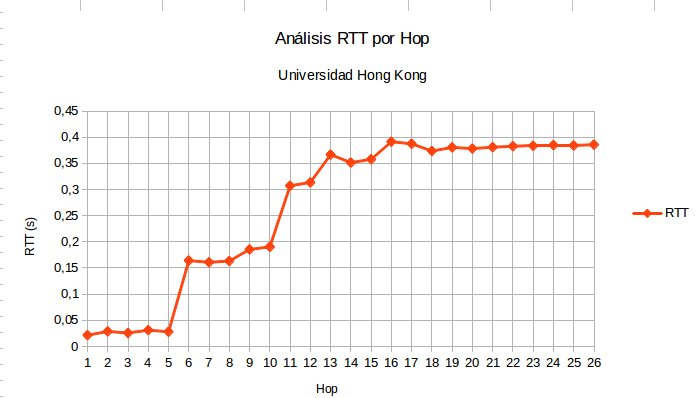
\includegraphics[width=1\textwidth]{graficos/rTT_HongKong.jpg}
\caption{RTT promedio por hop - Universidad de Hong Kong}
\label{hongkong_rtt}
\end{figure}

\begin{figure}[H]
\centering
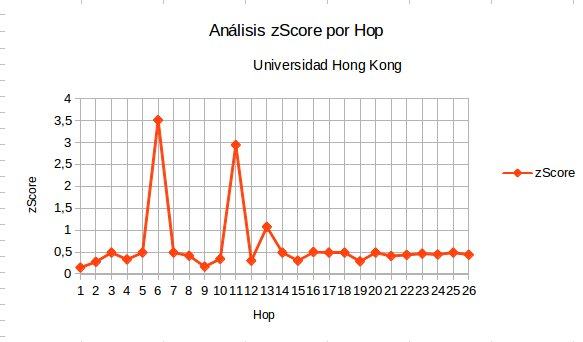
\includegraphics[width=1\textwidth]{graficos/zScore_HongKong.jpg}
\caption{zScore promedio por hop - Universidad de Hong Kong}
\label{hongkong_zs}
\end{figure}

Cómo hemos notado en las universidades anteriores, los $outliers$ detectados por el test de $Grubbs$ notamos que el $RTT$ crece abruptamente y que los $zScore$ tienen 
picos en ambos saltos.\\

Cómo nos ha sucedido para la Universidad en Francia, el salto 6 corresponde a un salto desde Argentina hacia Estados Unidos. Al existir una gran distancia entre ambos hosts 
nuestro test lo detecta.\\

Con respecto al salto 11 nos ha llamado la atención que la ubicación nos de en Estados Unidos. Los saltos anteriores tienen una $IP$ muy parecida y el $RTT$ acompaña la idea
que esos host se encuentren en América del Norte. Suponemos que el host del salto 11 no se encuentra en Estados Unidos dado que nos figura como $outlier$ en la distribución de 
los $\Delta$ $RTT$. Seguramente este host se encuentre en China y lo mismo para los host de los saltos siguientes que tienen un $RTT$ promedio mayor a 0,3 s. Por lo tanto
llegamos a la conclusión que en este salto existe un enlace submarino y nuevamente que no podemos tomar como válida la ubicación de la herramienta utilizada.\\

A continuación hemos trazado en un mapa la ruta de nuestro host hasta el host destino ubicado en Hong Kong - China:
\begin{figure}[H]
\centering
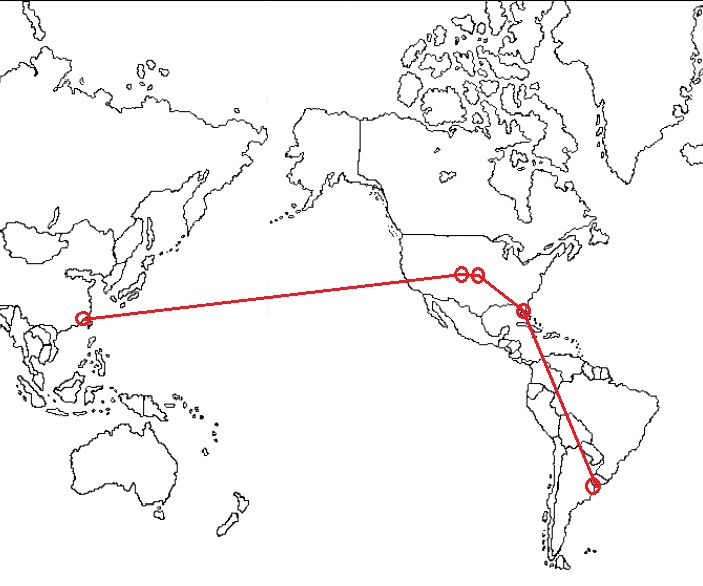
\includegraphics[width=0.8\textwidth]{graficos/mapa_hongKong.jpg}
\caption{Ruta en Internet - Universidad de Hong Kong}
\label{hongkong_zs}
\end{figure}
